\section{Introduction}
Solving partial differential equations (PDEs) underpins critical scientific advancements across diverse fields. Nowadays, enhanced computational capabilities combined with improved algorithms allow for high-fidelity numerical solutions to intricate problems using standard discretisation methods. For example, classical methods such as the finite element method (FEM) are used to solve the governing PDE. In this project, we are interested in solving the high-fidelity FEM model repeatedly. However, this could pose very high stress on the limited computational resources because solving high-fidelity models for various parameters usually involves computing many degrees of freedom for the solution. Hence, using the full-order model usually requires access to high-performance computing systems, which can be expensive. 

To address the issue, model order reduction (MOR) helps to alleviate the computational burden by identifying a lower dimensional representation of the parametric dependence of the high-fidelity model. The basic idea on which MOR is based is related to the fact that often the parametric dependence of the problem at hand has an intrinsic dimension much lower than the number of degrees of freedom associated to the governing high-fidelity solution \cite{shah2022finite}. There are two stages in an MOR procedure. The first one is an offline stage. During this stage, a large number of solutions (solved under different initialisations of parameters) are collected together to form a solution snapshot matrix. The MOR algorithm can then be run on the snapshot matrix, which identifies the most significant modes that form the reduced basis space. Stage two is an online stage where information regarding the reduced basis space is fully utilised, which allows for the computing of the projections of new high-fidelity solutions onto the lower intrinsic dimensions. 

We aim to develop a framework for data-driven MOR by combining Proper Orthogonal Decomposition (POD) with Artificial Neural Networks (ANN)\cite{hesthaven2018non}. The method involves identifying reduced basis space by performing POD, training the ANN with snapshots of PDE solutions as inputs, and using the trained ANN for a quick approximation of the solution field of a PDE. While offering data-driven efficiency and reducing reliance on high-fidelity FEM models, the trade-offs include a sacrifice in accuracy and extended training times for the ANN. The loss in accuracy was particularly evident in the vector field. Achieving a balance between accuracy and efficiency is crucial for the successful implementation of this approach.

To accelerate the runtime of the programme, this project leverages supercomputers through data-parallel computing, which divides tasks into smaller sub-tasks, allowing multiple processors to execute computations simultaneously. Both CPU and GPU-based parallelisation were utilised in the project. The CPU-based parallelisation involves distributing the computational workload across multiple CPU cores to accelerate the generation of data. This involves solving large-scale PDEs with the FEM library FEniCSx \cite{Baratta_DOLFINx_the_next_2023}, specifically for computing the FEM solutions for calculating the reduced basis functions in POD and for obtaining the ANN training data; In the context of ANN training, the GPU-based parallelisation was utilised with the help of TensorFlow. Partitions of the dataset are distributed to individual processors, each handling its subset of the dataset. Through distributed ANN training, parallel processing accelerates the learning process. The outputs during each training epoch (e.g. losses and gradients) are synchronised among processors. 


\begin{figure}[!h]
    \centering
    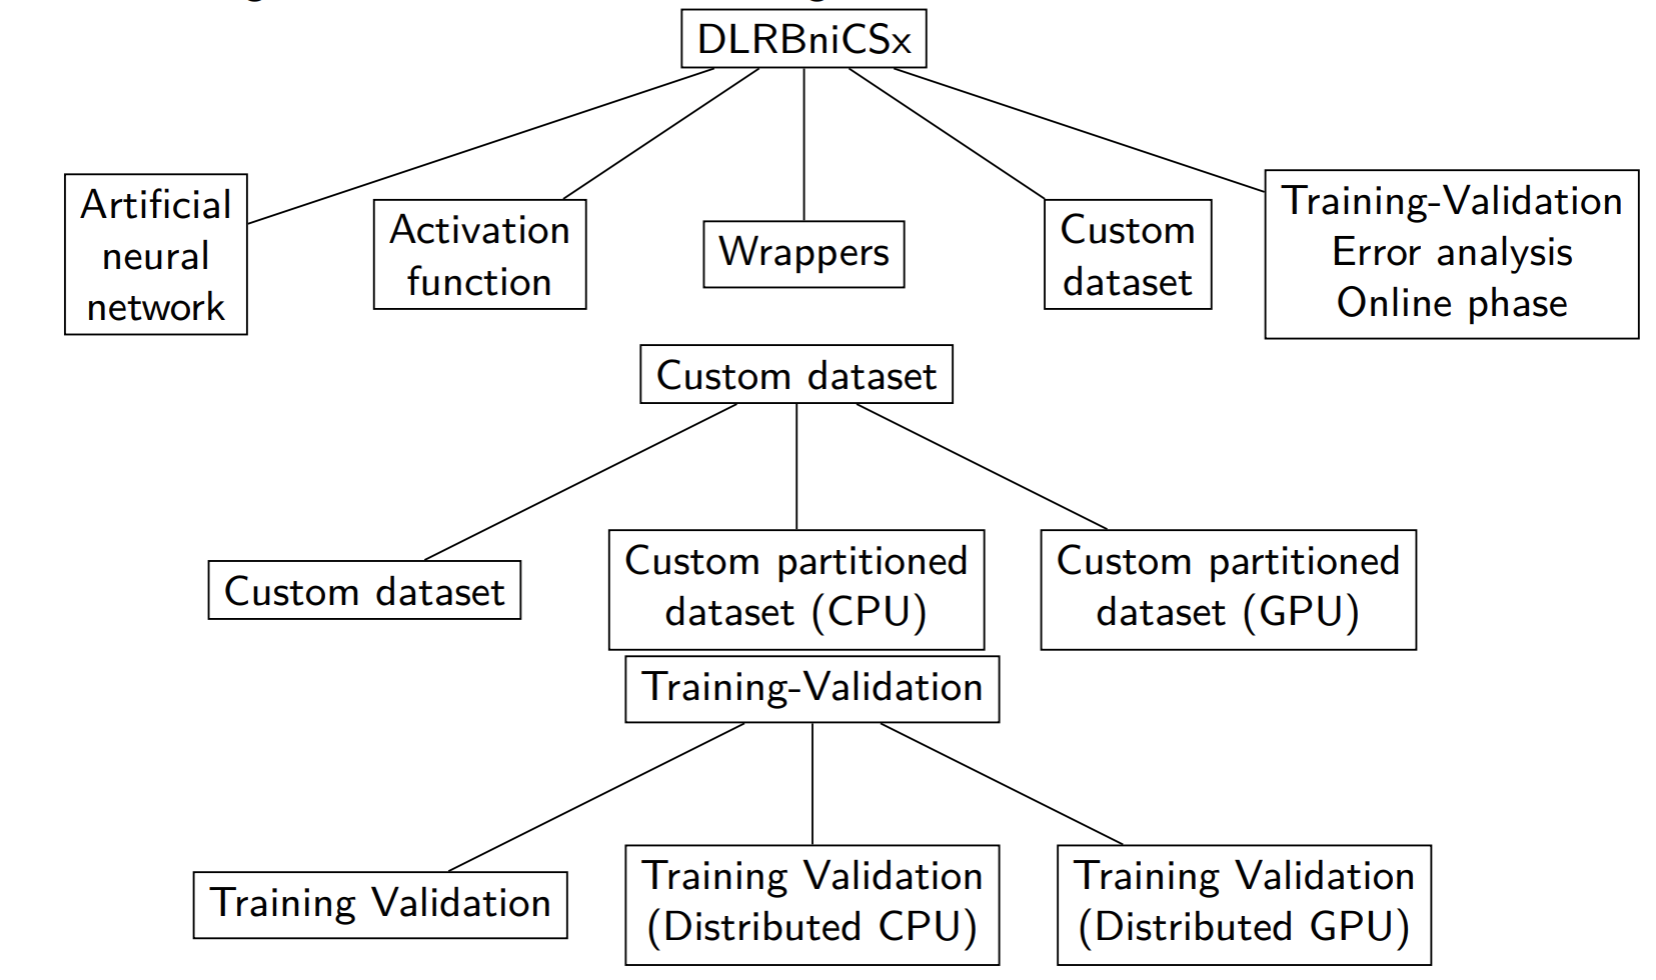
\includegraphics[width=0.7\linewidth]{parallel_fig/project_explain.png}
    \caption{Project outline}
    \label{fig:project_explain}
\end{figure}

\textcolor{red}{Notes for Nirav: could you please correct any misunderstandings I may have about the full picture of DLRBniCSx in the below paragraph? I was not so sure when drafting this paragraph, thank you.}
The entire process above is currently an ongoing work of the DLRBniCSx python package \cite{Nirav_Dlrbnicsx}, where an ANN-POD model has been developed for some types of PDE such as the linear/non-linear Poisson equations, the Navier-Stokes equations etc. DLRBniCSx is an open-source library currently built on PyTorch (for building and training ANN), RBniCSx \cite{Francesco_RBniCSx_2024}(for performing MOR), and FEniCSx (for solving PDEs using FEM), designed for deep learning-based reduced-order modelling. It offers a range of functionalities such as building the ANN, setting the activation functions, wrappers, and custom dataset management. The custom dataset feature encompasses both CPU and GPU partitioned datasets tailored for both Proper Orthogonal Decomposition (POD) and neural network training. Additionally, the library provides tools for training-validation error analysis. The whole picture of DLRBniCSx is shown in figure \ref{fig:project_explain}.

To enhance the usability of DLRBniCSx, a significant part of the project is dedicated to offering additional Tensorflow \cite{tensorflow2015-whitepaper} support to DLRBniCSx, and to designing a simple user interface based on Tensorflow. In addition, this project also focuses on the implementation of the mixed formulation for the Poisson equation, which included an extra vector term $\sigma$ that represented the flux of the scalar field in the Poisson equation. The parametrisation of PDEs incorporated changing variables in the governing equations, allowing for more flexibility in the system. In this report, we also explain the choices of the parameters through the MOR results and the range of parameters through the ANN results.  

Below is a summary of the workflow of this project, which will be discussed in greater depth in this report. In Section 2, we will introduce the governing equation of the mixed formulation for the Poisson equation and how the traditional finite element method is used to solve for the full-order solution. Section 3 focuses on the concept of parametrised 
PDEs and explain our choices of parameters focused on the project. In Section 4, the idea of MOR is explained in detail, and we will discuss the result and the effectiveness of MOR in reducing dimensionality, along with a more detailed explanation of the choice for parameterisation. The use of ANN will then be covered in Section 5, followed by a presentation of the numerical results in Section 6. Lastly, the concept of parallelisation is covered in Section 7.  

\begin{comment}
\begin{enumerate}
    \item \textbf{POD-ANN training phase:}
        \begin{enumerate}
            \item Use FEM to compute the sample solutions with different input parameters and obtain the snapshot matrix (incorporating parallelisation);
            \item Perform POD on the snapshot matrix to obtain the reduced basis space;
            \item Project the sample solutions on a reduced basis to obtain the training data;
            \item Train the ANN with the training dataset (incorporating parallelisation).
        \end{enumerate}

    \item \textbf{Prediction phase:}
        \begin{enumerate}
            \item Insert the input parameters to the trained ANN and obtain the predicted output on the reduced basis function space;
            \item Reconstruct the high-fidelity solution from the reduced basis output and the reduced basis functions.
        \end{enumerate} 
\end{enumerate}
%%%
\end{comment}

\newpage